% Shear stress along a bonded single lap for three overlaps, same load. Example 8.4.
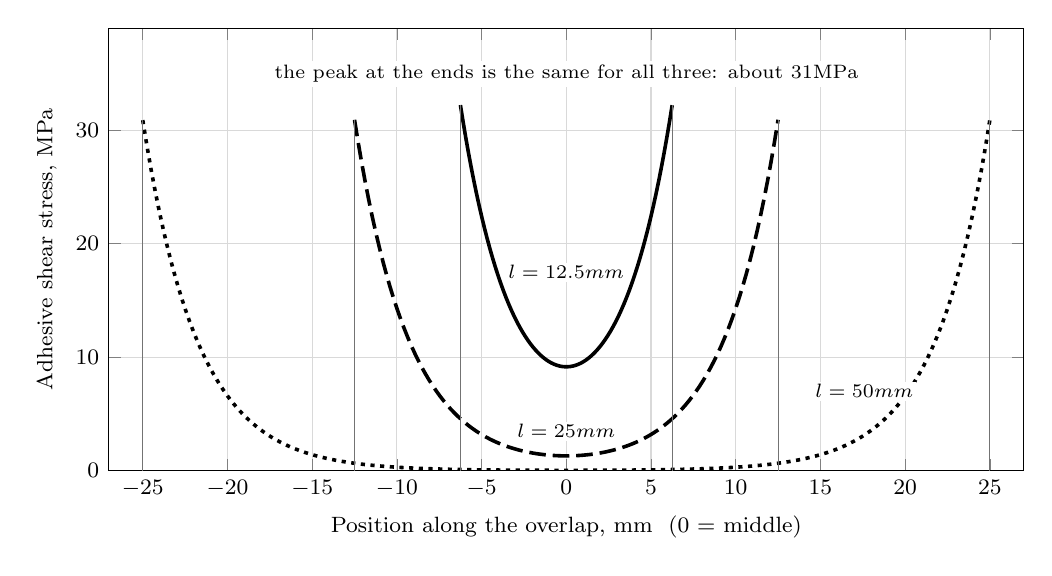
\begin{tikzpicture}
\begin{axis}[width=13.2cm,height=7.2cm,xmin=-27,xmax=27,ymin=0,ymax=39,
  xlabel={Position along the overlap, mm \ (0 = middle)},ylabel={Adhesive shear stress, MPa},
  label style={font=\footnotesize},tick label style={font=\footnotesize},grid=major,major grid style={black!15},clip=true]
% tau(x) = (P w / (2 b)) cosh(w x)/sinh(w l/2),  P=5000 N, b=25 mm, w=0.3090 /mm
\addplot[black,line width=1.3pt,domain=-6.25:6.25,samples=80] {30.90*cosh(0.3090*x)/sinh(0.3090*6.25)};
\addplot[black,line width=1.3pt,dash pattern=on 6pt off 2.5pt,domain=-12.5:12.5,samples=120] {30.90*cosh(0.3090*x)/sinh(0.3090*12.5)};
\addplot[black,line width=1.3pt,dash pattern=on 1.5pt off 2pt,domain=-25:25,samples=200] {30.90*cosh(0.3090*x)/sinh(0.3090*25)};
\addplot[black!55,line width=0.4pt] coordinates {(-6.25,0) (-6.25,32.2)}; \addplot[black!55,line width=0.4pt] coordinates {(6.25,0) (6.25,32.2)};
\addplot[black!55,line width=0.4pt] coordinates {(-12.5,0) (-12.5,30.9)}; \addplot[black!55,line width=0.4pt] coordinates {(12.5,0) (12.5,30.9)};
\addplot[black!55,line width=0.4pt] coordinates {(-25,0) (-25,30.9)}; \addplot[black!55,line width=0.4pt] coordinates {(25,0) (25,30.9)};
\node[font=\scriptsize,anchor=south,fill=white,inner sep=1pt] at (axis cs:0,16.6) {$l=\SI{12.5}{mm}$};
\node[font=\scriptsize,anchor=south,fill=white,inner sep=1pt] at (axis cs:0,2.6) {$l=\SI{25}{mm}$};
\node[font=\scriptsize,anchor=west,fill=white,inner sep=1pt] at (axis cs:14.5,7) {$l=\SI{50}{mm}$};
\node[font=\scriptsize,anchor=south,fill=white,inner sep=1.5pt] at (axis cs:0,33.8) {the peak at the ends is the same for all three: about \SI{31}{MPa}};
\end{axis}
\end{tikzpicture}
